	\section{Metadados} 
	
	Os sistemas de arquivos, como ambientes propícios para a recuperação de informações, têm na utilização de metadados a padronização das formas de representação e a possibilidade de garantia de interoperabilidade entre sistemas, favorecendo a integridade e a acessibilidade dos recursos informacionais de forma eficiente pelo usuário final. Os metadados são "dodos de dodos", ou seja, as informações essenciais sobre os arquivos armazenados, indispensáveis para fazer o gerenciamento de arquivos, indicando as características inerentes deles. A Tabela~\ref{tab:metadado} mostra os atributos encontrados em um metadado.
	
	\capstartfalse
	\begin{table} [htb]
		\caption{Elementos de metadadso}
		\centering
		\begin{tabular}{|l|l|} \hline
			\textbf{Informação} & \textbf{Descrição} \\ \hline
			
			Nome do arquivo		& O nome do arquivo, incluindo o caminho do diretório.\\ \hline
			Proprietário		& O identificador de usuário que é o dono do arquivo.\\ \hline
			Data de criação     & Data que o arquivo foi criado.\\ \hline
			Data de acesso		& Data de último acesso do arquivo. \\ \hline
			Data de atualização	& Data de última atualização feito sobre o arquivo. \\ \hline
			Tamanho				& Espaço ocupado pelo arquivo ao longo do disco. \\ \hline
			Tipo de arquivo		& indica se ele é uma pasta ou um arquivo normal.  \\ \hline
			Modo de acesso		& indica a permissão para acessar o arquivo. \\ \hline
			Bloqueio			& indica se o arquivo está bloqueado para acesso. \\ \hline
			Lista de servidores	& lista de todos os servidores que armazena partes do arquivo. \\ \hline
			
		\end{tabular}
		\label{tab:metadado}
	\end{table}
	\capstarttrue

	\section{Arquitetura do sistema}
	
	A arquitetura do SAD proposto neste artigo é composto por vários clientes e servidores distribuídos, onde cada um deles está conectado através de internet, como a Figura~\ref{fig:vis_sis} mostra resumidamente. Neste sistema, cada servidor se comporta como um disco rígido em sistema de RAID, armazenando distribuidamente as partes dos arquivos e paridades associadas.
	
	
	%O nosso objeivo neste artigo é a construção de um SAD baseado na computação em nuvem que possui menor \textit{overhead} de espaço, comparado a 200\% de método de replicação, sem degradar muito o performance e segurança de dados. 
	%Para isso, nós observamos em técnica de redundância usado na tecnologia RAID, onde consegue diminuir o espaço ocupado pela parte redundante com atribuição de paridade nos arquivos, ao invés de simples replicação. Na mesma tecnologia também foi 

	
	
	\begin{figure}[htb]
		\begin{center}
			
			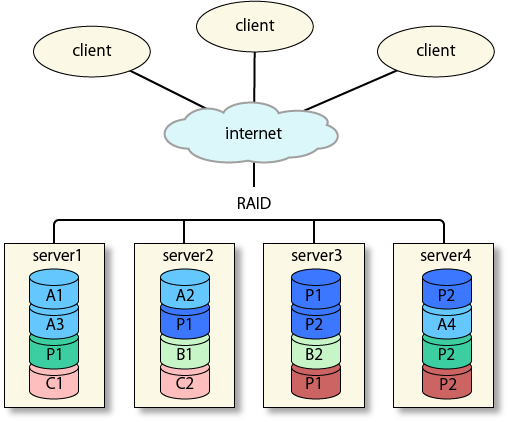
\includegraphics[clip,width=10.0cm]{images/image1.png}
			\caption{Visão geral do sistema}
			\label{fig:vis_sis}
		\end{center}
	\end{figure}
	
	
	
	\subsection{Servidor}
	
	Grupo de servidores que fazem armazenamento e gerenciamento de dados. \\
	
	Em um sistema de arquivos local, normalmente o metadado e o conteúdo de um arquivo são armazenados na mesma unidade de armazenamento. No caso de um SAD, como um arquivo pode ser armazenados distribuidamente entre servidores diferentes, os metadados são espalhados por vários servidores, tendo assim, a necessidade de fazer a busca para acessar em um determinado metadado. Obviamente essa busca consome recursos operacionais, relativamente alta por tratar de uma transmissão na rede.   
	\begin{figure}[htb]
		\begin{center}
			
			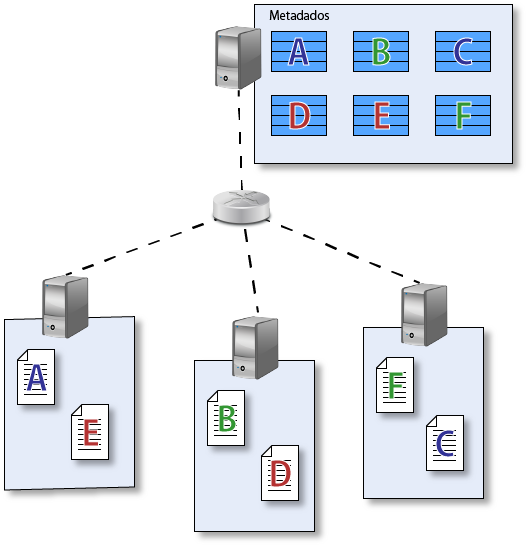
\includegraphics[clip,width=10.0cm]{images/image7.png}
			\caption{\textit{Name node} e \textit{data node}}
			\label{fig:namenode}
		\end{center}
	\end{figure}
	
	\subsubsection{\textit{Name node}}
	
	O \textit{name node} é o conjunto de servidores que gerencia as informações dos arquivos armazenados, em forma de metadado.
	Mantém na sua memória local a árvore de diretórios, o que indica localização lógica dos arquivos. Quando recebe uma solicitação de cliente por um arquivo, pesquisa a sua árvore de diretórios para identificar qual diretório que este arquivo se encontra. Como resultado da pesquisa obtém o metadado do arquivo referente, conseguindo descobrir a sua localização física, a lista dos todos os \textit{data nodes} que possuem as partes do arquivo. Assim, também gerencia as comunicações entre clientes e \textit{data nodes}, informando os clientes quais são os servidores que devem estabelecer a conexão para enviar ou receber um arquivo. 
	\\
	
	Por sua propriedade como um interface entre clientes e \textit{data nodes}, a ocorrência de alguma falha na operação ou indisponibilidade causada pela queda do servidor tem  enorme influencia na execução do sistema, podendo até resultar em parada total do sistema. Assim, é muito importante elaborar uma esquema para manter o \textit{name node} protegidos contra falhas ou queda total. Em nosso sistema usaremos a biblioteca BFT-SMaRt, que fornece tolerância a falha no serviço através de replicação por máquina de estado. 
	
	\subsubsection{\textit{Data node}}
	
	Parte que realiza o armazenamento de arquivos em si.
	
	\subsection{Cliente}
	Programa cliente que é executado no computador de um usuário. 
	\\
	
	O programa cliente é capaz de dividir um arquivo em vários pedaços e gerar paridades. Por consequência, também é capaz de reconstruir um arquivo a partir de partes divididos. A Figura~\ref{fig:img6} mostra o procedimento.
	\begin{figure}[htb]
		\begin{center}
			
			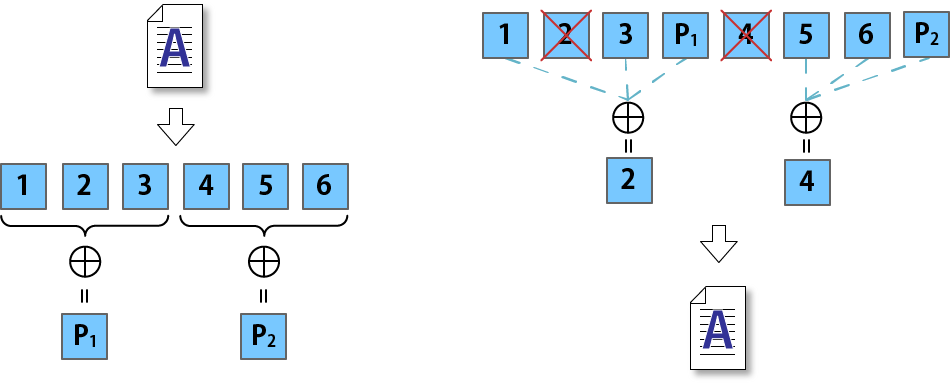
\includegraphics[clip,width=15.0cm]{images/image6.png}
			\caption{Geração de paridade}
			\label{fig:img6}
		\end{center}
	\end{figure}
	
	Para assegurar a disponibilidade do sistema, é interessante que o usuário tenha acesso ao um arquivo mesmo que algum dos seus fragmentos de dado esteja indisponível por uma razão qualquer, recuperando o arquivo íntegro a partir de fragmentos disponíveis neste momento.\\
	
	Quando um cliente percebe que o arquivo que solicitou apresenta  
	A Figura~\ref{fig:img2} mostra esquema para recuperar um arquivo no lado do cliente.
	
	\begin{figure}[htb]
		\begin{center}
			
			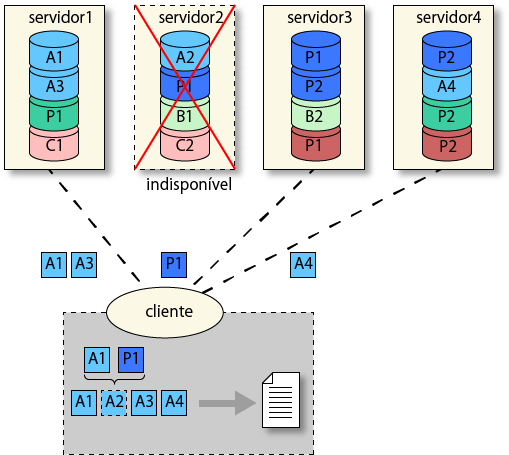
\includegraphics[clip,width=10.0cm]{images/image2.png}
			\caption{Recuperando um arquivo de uma falha}
			\label{fig:img2}
		\end{center}
	\end{figure}
	
	\section{Operações}
	
	Nesta seção serão apresentadas as operações básicas que o SAD executa. Estas operações podem ser divididos em dois grupos dependendo dos entidades envolvidos na operação executada. Um deles é entre cliente e servidor, onde consiste das operações que podem ser encontradas em sistemas de arquivos em geral, focalizadas em fornecer um serviço de armazenamento de dados. Outro tipo é as operações que ocorrem entre servidores, voltadas para gerenciamento do serviço. Este tipo de operação não pode ser percebido por usuário, mantendo algumas transparências.
	
	
	%Os protocolos neste sistema indicam os tipos de mensagens que vai ser trocado entre cliente/servidor ou servidor/servidor. 
	
	\subsection{Cliente-Servidor}
	
	É um conjunto de operações semelhantes a que são implementadas em um sistema de arquivos local, aquele que é integrado na maioria dos sistemas operacionais comuns. Composto pelas operações sobre arquivos e pastas e suas execuções podem ocorrer entre cliente e \textit{name node} ou cliente e \textit{data node}.
	
	\subsubsection{Criar arquivos}
	
	Quando um cliente deseja criar um arquivo dentro de um SAD, primeiramente deve enviar para servidor do tipo \textit{name node} o metadado referente ao arquivo, o que contem as informações essenciais como nome, diretório, tamanho e entre outros. No lado do servidor, recebendo o metadado do arquivo a ser criado, extrai dele o nome e diretório do arquivo. 
	
	\subsubsection{Abrir arquivos}
	
	Abrir um arquivo existente provavelmente vai ser uma das tarefas mais usado no sistema. Geralmente é composto por três procedimentos básicos. Esta operação inicia pegando como referencia o nome e o diretório do arquivo, e procura por nome neste diretório. É muito importante que a busca pelo arquivo tenha uma boa eficiência, pois uma vez que este procedimento é executado muitas vezes e normalmente um servidor de grande porte possui  diretórios com milhares entradas encontrados dentro deles. Assim, a escolha do estrutura de dados para diretórios pode influenciar criticamente no desempenho do sistema. Depois de encontrar o arquivo desejado, será verificado algumas condições para decidir se o arquivo pode ser aberto mesmo. Uma condição é se o arquivo não esteja bloqueado por outros usuários, impedindo que seja aberto no momento. Outra é se o usuário que solicitou o acesso por este arquivo possui a permissão para fazer isso. Passando por checagem das permissões de acesso, finalmente o servidor envia uma resposta para cliente, indicando os servidores que armazenam cada pedaços do arquivo.
	 
	\subsubsection{Deletar arquivos}
	Deletar um arquivo vai seguir procedimentos semelhantes a operação de abrir arquivo. Em primeiro lugar recebe o nome e diretório do arquivo a ser apagado. Faz a busca pela árvore de diretórios para achar o diretório requisitado, e chegando em diretório correto, procura o arquivo por nome. Quando encontra o arquivo desejado, verifica se está satisfazendo as condições para efetuar a operação, checando a permissão de acesso e estado de bloqueio do arquivo.  
	
	\subsubsection{Fechar um arquivo aberto}
	
	Fechar o arquivo aberto por um cliente.
	
	\subsubsection{Editar um arquivo}
	
	Fazer alteração no arquivo armazenado.
	
	\subsubsection{Modificar metadado}
	
	Permite fazer alterações sobre as informações do arquivo, editando diretamente o metadado associado.
	
	
	\subsection{Servidor-Servidor}
	São operações ocorridos entre \textit{name node} e \textit{data node}, com função de gerenciamento de SAD.
	
	\subsubsection{Receber arquivo criado}
	
	Na operação de criar arquivo, o \textit{name node} define quais \textit{data nodes} vão ser utilizados para armazenar os fragmentos de arquivo a ser criado, calculando a melhor forma para distribuir igualmente a carga entre os \textit{data nodes}. Dessa forma, além de informar o cliente quais são os servidores que deve enviar os dados, deve avisar os \textit{data nodes} que vai chegar dados enviados pelo cliente.
	
	\subsubsection{Apagar arquivo deletado}
	
	Deleta os dados pertencentes ao arquivo solicitado para exclusão.
	
	\subsubsection{Transferir dados entre servidores}
	
	Transferência de arquivos entre \textit{data nodes}.
	
	
	
	